\usepackage[utf8x]{inputenc}
\usepackage[T1]{fontenc}
\usepackage[ngerman]{babel}
\usepackage{stmaryrd}
\usepackage{amsfonts}
\usepackage{amssymb}
\usepackage{amsmath}
\usepackage{microtype}

\usepackage{listings}
\usepackage{color}
\usepackage{pxfonts}

\definecolor{mygreen}{RGB}{51,141,120}
\definecolor{myblue}{RGB}{0,128,180}
\definecolor{myviolet}{RGB}{118,0,118}

\lstset{ %
  language=Haskell,
  backgroundcolor=\color{white},         % choose the background color
  basicstyle=\ttfamily\footnotesize,     % size of fonts used for the code
  numbers=none,
  breaklines=true,                       % automatic line breaking only at whitespace
  captionpos=b,                          % sets the caption-position to bottom
  commentstyle=\color{mygreen},    % comment style
  escapeinside={\%*}{*)},                % if you want to add LaTeX within your code
  keywordstyle=\color{myblue}\bfseries, % keyword style
  stringstyle=\color{myviolet},    % string literal style
  frame=single,
  tabsize=2
}
\usepackage{tikz}
\usetikzlibrary{
  arrows,
  shapes.misc,
  shapes.arrows,
  chains,
  matrix,
  positioning,
  scopes,
  decorations.pathmorphing,
  shadows,
  backgrounds
}


\usetheme[%
  %cmyk,%<cmyk/rgbprint>,          Auswahl des Farbmodells
  orange,%<blue/orange/green/violet> Auswahl des Sekundärfarbklangs
  %dark,%<light,medium>        Auswahl der Helligkeit
  %colorhead,%    Farbig hinterlegte Kopfleiste
  %colorfoot,%    Farbig hinterlegt Fußleiste auf Titelseite
  %colorblocks,%   Blöcke Farbig hinterlegen
  %nopagenum,%    Keine Seitennumer in Fußzeile
  %nodate,%       Kein Datum in Fußleiste
  %tocinheader,%   Inhaltsverzeichnis in Kopfleiste
  %tinytocinheader,% kleines Kopfleisten-Inhaltsverzeichnis
  %widetoc,%      breites Kopfleisten-Inhaltsverzeichnis
  %narrowtoc,%    schmales Kopfleisten-Inhaltsverzeichnis
  %nosubsectionsinheader,%  Keine subsections im Kopfleisten-Inhaltsverzeichnis
  %nologoinfoot,% Kein Logo im Fußbereich darstellen
  ]{tubs}

\titlegraphic[scaled]{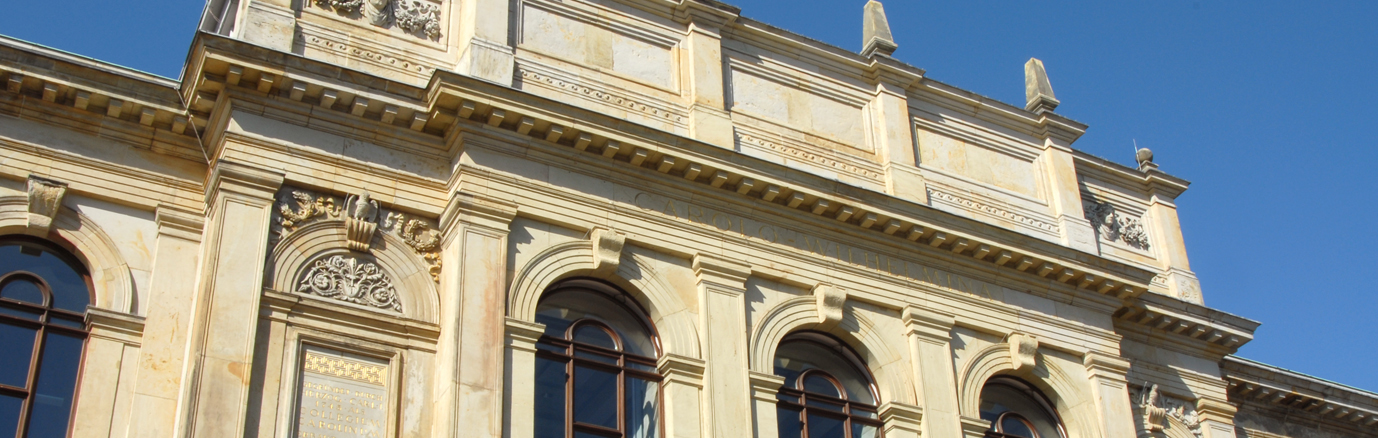
\includegraphics{img/titlepicture.jpg}}
\logo{
\includegraphics{img/logo_mit_text.pdf}}

\AtBeginSection[]{
  \begin{frame}[noframenumbering] 
  		\scriptsize
  		\frametitle{Überblick}  
  		\tableofcontents[currentsection, hideallsubsections]
  \end{frame}
}

\AtBeginSubsection[]{
  \begin{frame}[noframenumbering]
    	\scriptsize 
  		\frametitle{\insertsectionhead - \insertsubsectionhead} 
  		\tableofcontents[ 
  			currentsubsection, 
  		    sectionstyle=show/hide, 
  		   	subsectionstyle=show/shaded/hide] 
  \end{frame}
}
